\section{Special Attack}
\begin{frame}{$\alpha-$Reflection.}
\begin{itemize}
    \item Previous Works on Reflection attacks
    \item It has been applied on some ciphers and hash functions with Feistel construction 
    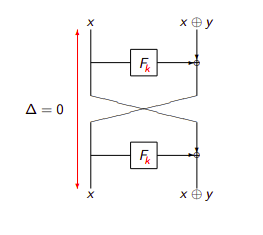
\includegraphics[scale=0.5]{Presentation/alpha-Intro.png}
    \item Using Probabilistic approach rather than deterministic approach.
\end{itemize}
    
\end{frame}
\begin{frame}{$\alpha-$Reflection.}
\begin{itemize}

    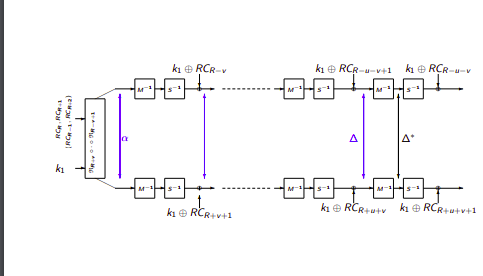
\includegraphics[scale = 0.5]{Presentation/Pc_alpha.png}
    \item To maximize $P_{c}$, we use
    \begin{enumerate}
        \item Cancellation idea.
        \item Branch and Bound Algorithm.
    \end{enumerate}
\end{itemize}
    
\end{frame}
\begin{frame}{Cancellation Idea}
    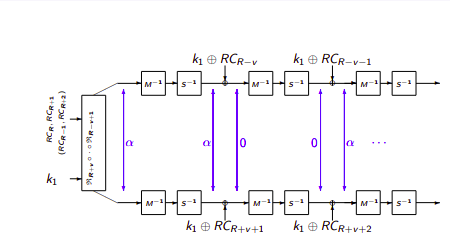
\includegraphics[scale=0.75]{Presentation/Canccellation.png}
    \begin{itemize}
        \item $\rho =Pr_{x}[S(X) \oplus S(X+ \alpha)]=M^{-1}(\alpha)$ there is an iterative characterstic over four rounds of PRINCE cypher.
    \end{itemize}
\end{frame}
\begin{frame}{Cancellation idea vs Branch and Bound Algorithm}
    \begin{itemize}
        \item Cancellation Idea
        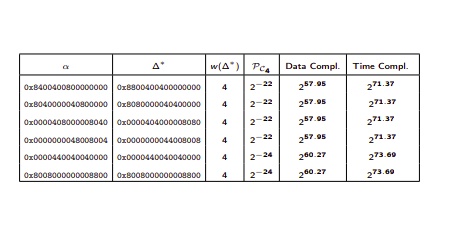
\includegraphics[scale=0.5]{Presentation/Canc_alpha.png}
        \item Branch and Bound Algorithm
        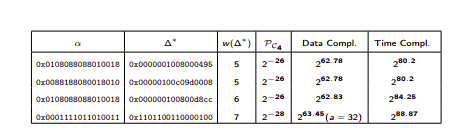
\includegraphics[scale=0.5]{Presentation/Bnb_alpha.png}
    \end{itemize}
\end{frame}
\begin{frame}{$\alpha-$Reflection Property}
\begin{itemize}
    \item PRINCE Cipher has a symmetric nature.
    \item $RC_{i} \oplus RC_{11-i}=$ constant, where RC is round constant, and $0\geq i\leq 11$
    \item For a key($k_{0}||k^{'}_{0}||k_{1}$ 
    \\
    $D_{k_{0}||k_{0}^{'}||k_{1}}$(.)=$E_{k_{0},k^{'}_{0},k_{1}+\alpha}$()
\end{itemize}
    
\end{frame}
\begin{frame}{Impact of construction implementing $\alpha-$Reflection Property}
\begin{itemize}
    \item If the decomposition of core cipher is independent from the key, then use the attack consisting of two plaintext-ciphertext pairs $(m,c) \quad (m^{'},c^{'})$
    such that $m \oplus c=m^{'} \oplus c^{'}$
    \\
    where, $m^{'}=E^{-1}_{k_{0},k^{'}_{0},k_{1}}(m \oplus k_{0} \oplus k_{2})$
    \item Such a collision could be found if the attacker has an access to $2^{\frac{n+1}{2}}$ known plaintext-ciphertext pairs and provides a value of $k_{0} \oplus k_{2}$
\end{itemize}
    
\end{frame}
\begin{frame}{Impact of construction implementing $\alpha-$Reflection Property}
\begin{itemize}
    \item A more relevant attack method consists
in using the fact that the core cipher may have a peculiar cycle decomposition for some weak key.
\item It is worth noticing that this attack applies to
DESX and allows to detect the use of the four weak keys of DES for which DES is an involution.
\item For the class of keys such that $k^{'}_{1} = k_{1} \oplus \alpha$, it holds that $F^{−1}_{(k_{1}||k^{'}_{1})} =F_{(k1||k^{'}_{1})}$, that is, the core cipher is an involution. This class of weak keys can then be
easily detected.
\end{itemize}
    
\end{frame}